\input{preamble.tex}

\begin{document}
\pagestyle{fancy}
\fancyhead[L]{Seconde}
\fancyhead[C]{\textbf{DS n°1 — Ensembles de nombres}}
\fancyhead[R]{\today}

\reversemarginpar

\null\vspace{-30pt}
Nom / Prénom : \\

Consignes particulières : 
\begin{itemize}[label=$\bullet$]
	\item 
	La calculatrice est {interdite}.
	\item 
	Les exercices \ref{exe:1} et \ref{exe:2} peuvent être fait entièrement sur la feuille d'évaluation. Écrire son nom avant de rendre le sujet pour qu'ils soient corrigés.
	\item 
	Toute trace de recherche est prise en compte.
	\item 
	L'abbréviation $\tq$ signifie ``tel que''.
\end{itemize}

\hrule

\exe{2}{
Compléter les affirmations suivantes :
\begin{enumerate}
\item $\N \dots \Z \dots \D \dots \Q \dots \R$.
\item Le plan cartésien est l'ensemble $\{ (\dots, \dots) \tq x \in \dots \et y \in \dots \}$.
\end{enumerate}
}{exe:1}{

}

\exe{4}{
On donne $\sqrt{2} \approx 1,414~213$. \\
On considère le point $H(\sqrt{2} ; 1)$. 

\begin{enumerate}
\item Proposer un encadrement à $10^{-1}$ près de l'abscisse de $H$.
\item Placer dans le repère ci-dessous les points $E(x_E,2)$ et $F(x_F,2)$ tels que
$x_E$ est la borne inférieure de l'encadrement proposé et $x_F$ sa borne supérieure.
\end{enumerate}

\begin{center}
	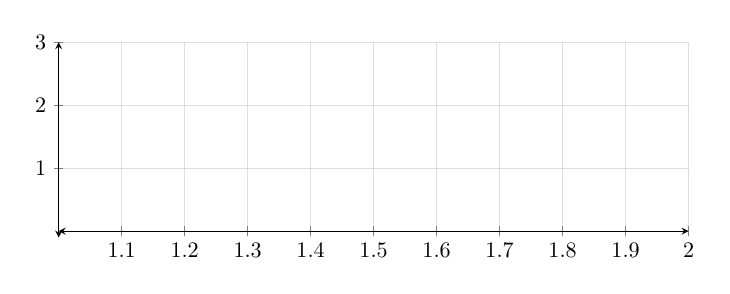
\begin{tikzpicture}[>=stealth, scale=.8]
		\begin{axis}[xmin = 1, xmax=2, ymin=-0.1, ymax=3, axis x line=middle, axis y line=middle, axis line style=<->, xlabel={}, ylabel={}, grid=both, grid style = {opacity=.5}, clip=false, xtick distance = 0.1, ytick distance=1, x=10cm, y=1cm]
		\end{axis}
	\end{tikzpicture}
\end{center}
}{exe:2}{
	
}
	
\exe{4}{
On considère les points $A\left(4;\frac23 \right)$ et $B\left(3;-\frac43 \right)$.
\begin{enumerate}
\item Calculer la \textbf{valeur exacte} de la distance $AB$.
\item Calculer les coordonnées du point $M(x_M, y_M)$, milieu du segment $[AB]$.
\item Donner les \textbf{plus petits} ensembles de nombres auxquels $x_I$ et $y_I$ appartiennent.
\end{enumerate}
\textit{``plus petit'' est entendu au sens de l'inclusion}
}{exe:3}{

}
	
\exe{4}{
\begin{multicols}{2}
On considère le triangle de sommets :
		\[ A(6;-3), \qquad B(4; 16), \quad \text{et} \quad C(-2 ; 0).\]
	
	\begin{enumerate}
		\item Calculer les valeurs suivantes.
		\begin{enumerate}[label=\roman*)]
			\item $AB^2$
			\item $AC^2$
			\item $BC^2$
		\end{enumerate}
		\item Que dire du triangle $ABC$ ? Justifier.
	\end{enumerate}

	%\hfill
	%Aide aux calculs
	\def\arraystretch{1.1}
	\setlength\tabcolsep{15pt}
	%\hfill
	\begin{center}
	\begin{tabular}{|c|c|}\hline
		$n$ & $n^2$ \\ \hline
		11 & 121 \\ \hline
		12 & 144 \\ \hline
		13 & 169 \\ \hline
		14 & 196 \\ \hline
		15 & 225 \\ \hline
		16 & 256 \\ \hline
		17 & 289 \\ \hline
		18 & 324 \\ \hline
		19 & 361 \\ \hline
		20 & 400 \\ \hline
	\end{tabular}
	\hspace{15pt}
	\begin{tabular}{|c|c|}\hline
		$n$ & $n^2$ \\ \hline
		21 & 441 \\ \hline
		22 & 484 \\ \hline
		23 & 529 \\ \hline
		24 & 576 \\ \hline
		25 & 625 \\ \hline
		26 & 676 \\ \hline
		27 & 729 \\ \hline
		28 & 784 \\ \hline
		29 & 841 \\ \hline
		30 & 900 \\ \hline
	\end{tabular}
	\end{center}
\end{multicols}
}{exe:4}{

}
%	\begin{center}
%	\begin{tikzpicture}[>=stealth, scale=1]
%		\begin{axis}[axis x line=middle, axis y line=middle, axis line style=<->, xlabel={}, ylabel={}, grid=both, grid style = {opacity=.5}, x=.7cm, y=.7cm]			
%			\addplot[blue, mark=*, mark size = 1] (\xA,\yA) node[above] {$A$};
%			\addplot[red, mark=*, mark size = 1] (\xB,\yB) node[right] {$B$};
%			\addplot[green, mark=*, mark size = 1] (\xC,\yC) node[left] {$C$};
%			
%			\draw[-, thick] (axis cs:\xA,\yA) -- (axis cs:\xB,\yB) -- (axis cs:\xC,\yC) -- (axis cs:\xA,\yA);
%		\end{axis}
%	\end{tikzpicture}
%	\end{center}
%	
%	\begin{enumerate}
%		\item%[2.] 
%			\begin{align*}
%				AB^2 &= \norm{A-B}^2 = \norm{(-6 ; 9)}^2 = 36 + 81 = 117, \\
%				AC^2 &= \norm{A-C}^2 = \norm{(12 ; 8)}^2 = 144 + 64 = 208, \\
%				BC^2 &= \norm{B-C}^2 = \norm{(18 ; -1)}^2 = 324 + 1 = 325.
%			\end{align*}
%		\item%[3.] 
%		D'après la réciproque du théorème de Pythagore, le triangle est rectangle en $A$ car $BC^2 = AB^2 + AC^2$.
%	\end{enumerate}
%}

\exe{}{
(Exercice bonus) \\
On considère les points $A \left ( \frac{-3}{2} ; 4 \right )$ et $B \left ( 7 ; \frac{-3}5 \right)$. 
Calculer les coordonnées du point $C$ afin que $B$ soit le milieu du segment $[AC]$
}{exe:5}{

}

%%%%%%%%%%%%

%\newpage
%\fancyhead[C]{\textbf{Solutions}}
%\shipoutAnswer

\end{document}
